\documentclass[11pt,table]{article}

\usepackage[table]{xcolor}

\usepackage[breakable]{tcolorbox}
\usepackage{parskip} % Stop auto-indenting (to mimic markdown behaviour)

\usepackage{iftex}
\ifPDFTeX
\usepackage[T1]{fontenc}
\usepackage{mathpazo}
\else
\usepackage{fontspec}
\fi

% Basic figure setup, for now with no caption control since it's done
% automatically by Pandoc (which extracts ![](path) syntax from Markdown).
\usepackage{graphicx}
% Maintain compatibility with old templates. Remove in nbconvert 6.0
\let\Oldincludegraphics\includegraphics
% Ensure that by default, figures have no caption (until we provide a
% proper Figure object with a Caption API and a way to capture that
% in the conversion process - todo).
\usepackage{caption}
\DeclareCaptionFormat{nocaption}{}
\captionsetup{format=nocaption,aboveskip=0pt,belowskip=0pt}

\usepackage{float}
\floatplacement{figure}{H} % forces figures to be placed at the correct location


%\usepackage{xcolor} % Allow colors to be defined
\usepackage{enumerate} % Needed for markdown enumerations to work
\usepackage{geometry} % Used to adjust the document margins
\usepackage{amsmath} % Equations
\usepackage{amssymb} % Equations
\usepackage{textcomp} % defines textquotesingle
% Hack from http://tex.stackexchange.com/a/47451/13684:
\AtBeginDocument{%
	\def\PYZsq{\textquotesingle}% Upright quotes in Pygmentized code
}
\usepackage{upquote} % Upright quotes for verbatim code
\usepackage{eurosym} % defines \euro
\usepackage[mathletters]{ucs} % Extended unicode (utf-8) support
\usepackage{fancyvrb} % verbatim replacement that allows latex
\usepackage{grffile} % extends the file name processing of package graphics 
% to support a larger range
\makeatletter % fix for old versions of grffile with XeLaTeX
\@ifpackagelater{grffile}{2019/11/01}
{
	% Do nothing on new versions
}
{
	\def\Gread@@xetex#1{%
		\IfFileExists{"\Gin@base".bb}%
		{\Gread@eps{\Gin@base.bb}}%
		{\Gread@@xetex@aux#1}%
	}
}
\makeatother
\usepackage[Export]{adjustbox} % Used to constrain images to a maximum size
\adjustboxset{max size={0.9\linewidth}{0.9\paperheight}}

% The hyperref package gives us a pdf with properly built
% internal navigation ('pdf bookmarks' for the table of contents,
% internal cross-reference links, web links for URLs, etc.)
\usepackage{hyperref}
% The default LaTeX title has an obnoxious amount of whitespace. By default,
% titling removes some of it. It also provides customization options.
\usepackage{titling}
\usepackage{longtable} % longtable support required by pandoc >1.10
\usepackage{booktabs}  % table support for pandoc > 1.12.2
\usepackage[inline]{enumitem} % IRkernel/repr support (it uses the enumerate* environment)
\usepackage[normalem]{ulem} % ulem is needed to support strikethroughs (\sout)
% normalem makes italics be italics, not underlines
\usepackage{mathrsfs}
\usepackage{tikz}

% Colors for the hyperref package
\definecolor{urlcolor}{rgb}{0,.145,.698}
\definecolor{linkcolor}{rgb}{.71,0.21,0.01}
\definecolor{citecolor}{rgb}{.12,.54,.11}

% ANSI colors
\definecolor{ansi-black}{HTML}{3E424D}
\definecolor{ansi-black-intense}{HTML}{282C36}
\definecolor{ansi-red}{HTML}{E75C58}
\definecolor{ansi-red-intense}{HTML}{B22B31}
\definecolor{ansi-green}{HTML}{00A250}
\definecolor{ansi-green-intense}{HTML}{007427}
\definecolor{ansi-yellow}{HTML}{DDB62B}
\definecolor{ansi-yellow-intense}{HTML}{B27D12}
\definecolor{ansi-blue}{HTML}{208FFB}
\definecolor{ansi-blue-intense}{HTML}{0065CA}
\definecolor{ansi-magenta}{HTML}{D160C4}
\definecolor{ansi-magenta-intense}{HTML}{A03196}
\definecolor{ansi-cyan}{HTML}{60C6C8}
\definecolor{ansi-cyan-intense}{HTML}{258F8F}
\definecolor{ansi-white}{HTML}{C5C1B4}
\definecolor{ansi-white-intense}{HTML}{A1A6B2}
\definecolor{ansi-default-inverse-fg}{HTML}{FFFFFF}
\definecolor{ansi-default-inverse-bg}{HTML}{000000}

% common color for the border for error outputs.
\definecolor{outerrorbackground}{HTML}{FFDFDF}

% commands and environments needed by pandoc snippets
% extracted from the output of `pandoc -s`
\providecommand{\tightlist}{%
	\setlength{\itemsep}{0pt}\setlength{\parskip}{0pt}}
\DefineVerbatimEnvironment{Highlighting}{Verbatim}{commandchars=\\\{\}}
% Add ',fontsize=\small' for more characters per line
\newenvironment{Shaded}{}{}
\newcommand{\KeywordTok}[1]{\textcolor[rgb]{0.00,0.44,0.13}{\textbf{{#1}}}}
\newcommand{\DataTypeTok}[1]{\textcolor[rgb]{0.56,0.13,0.00}{{#1}}}
\newcommand{\DecValTok}[1]{\textcolor[rgb]{0.25,0.63,0.44}{{#1}}}
\newcommand{\BaseNTok}[1]{\textcolor[rgb]{0.25,0.63,0.44}{{#1}}}
\newcommand{\FloatTok}[1]{\textcolor[rgb]{0.25,0.63,0.44}{{#1}}}
\newcommand{\CharTok}[1]{\textcolor[rgb]{0.25,0.44,0.63}{{#1}}}
\newcommand{\StringTok}[1]{\textcolor[rgb]{0.25,0.44,0.63}{{#1}}}
\newcommand{\CommentTok}[1]{\textcolor[rgb]{0.38,0.63,0.69}{\textit{{#1}}}}
\newcommand{\OtherTok}[1]{\textcolor[rgb]{0.00,0.44,0.13}{{#1}}}
\newcommand{\AlertTok}[1]{\textcolor[rgb]{1.00,0.00,0.00}{\textbf{{#1}}}}
\newcommand{\FunctionTok}[1]{\textcolor[rgb]{0.02,0.16,0.49}{{#1}}}
\newcommand{\RegionMarkerTok}[1]{{#1}}
\newcommand{\ErrorTok}[1]{\textcolor[rgb]{1.00,0.00,0.00}{\textbf{{#1}}}}
\newcommand{\NormalTok}[1]{{#1}}

% Additional commands for more recent versions of Pandoc
\newcommand{\ConstantTok}[1]{\textcolor[rgb]{0.53,0.00,0.00}{{#1}}}
\newcommand{\SpecialCharTok}[1]{\textcolor[rgb]{0.25,0.44,0.63}{{#1}}}
\newcommand{\VerbatimStringTok}[1]{\textcolor[rgb]{0.25,0.44,0.63}{{#1}}}
\newcommand{\SpecialStringTok}[1]{\textcolor[rgb]{0.73,0.40,0.53}{{#1}}}
\newcommand{\ImportTok}[1]{{#1}}
\newcommand{\DocumentationTok}[1]{\textcolor[rgb]{0.73,0.13,0.13}{\textit{{#1}}}}
\newcommand{\AnnotationTok}[1]{\textcolor[rgb]{0.38,0.63,0.69}{\textbf{\textit{{#1}}}}}
\newcommand{\CommentVarTok}[1]{\textcolor[rgb]{0.38,0.63,0.69}{\textbf{\textit{{#1}}}}}
\newcommand{\VariableTok}[1]{\textcolor[rgb]{0.10,0.09,0.49}{{#1}}}
\newcommand{\ControlFlowTok}[1]{\textcolor[rgb]{0.00,0.44,0.13}{\textbf{{#1}}}}
\newcommand{\OperatorTok}[1]{\textcolor[rgb]{0.40,0.40,0.40}{{#1}}}
\newcommand{\BuiltInTok}[1]{{#1}}
\newcommand{\ExtensionTok}[1]{{#1}}
\newcommand{\PreprocessorTok}[1]{\textcolor[rgb]{0.74,0.48,0.00}{{#1}}}
\newcommand{\AttributeTok}[1]{\textcolor[rgb]{0.49,0.56,0.16}{{#1}}}
\newcommand{\InformationTok}[1]{\textcolor[rgb]{0.38,0.63,0.69}{\textbf{\textit{{#1}}}}}
\newcommand{\WarningTok}[1]{\textcolor[rgb]{0.38,0.63,0.69}{\textbf{\textit{{#1}}}}}

\newcommand{\R}{\mathbb{R}}

% Define a nice break command that doesn't care if a line doesn't already
% exist.
\def\br{\hspace*{\fill} \\* }
% Math Jax compatibility definitions
\def\gt{>}
\def\lt{<}
\let\Oldtex\TeX
\let\Oldlatex\LaTeX
\renewcommand{\TeX}{\textrm{\Oldtex}}
\renewcommand{\LaTeX}{\textrm{\Oldlatex}}
% Document parameters
% Document title
\title{Ejercicios Programación Lineal}


\usepackage{mdframed}


\newenvironment{problem}[2][Problem]
{ \begin{mdframed}[backgroundcolor=gray!20] \textbf{#1 #2} \\ }
	{  \end{mdframed} }

\newenvironment{question}[2][Question]
{ \begin{mdframed}[backgroundcolor=gray!20] \textbf{#1 #2} \\ }
	{  \end{mdframed} }

% Define solution environment
\newenvironment{solution}
{\textit{Solución}}
{}


\usepackage{fancyhdr} % Headers and footers
\pagestyle{fancy} % All pages have headers and footers
\fancyhead{}\renewcommand{\headrulewidth}{0pt} % Blank out the default header
\fancyfoot[L]{} % Custom footer text
\fancyfoot[C]{} % Custom footer text
\fancyfoot[R]{\thepage} % Custom footer text
\newcommand{\note}[1]{\marginpar{\scriptsize \textcolor{red}{#1}}} % Enables comments in red on margin



% Pygments definitions
\makeatletter
\def\PY@reset{\let\PY@it=\relax \let\PY@bf=\relax%
	\let\PY@ul=\relax \let\PY@tc=\relax%
	\let\PY@bc=\relax \let\PY@ff=\relax}
\def\PY@tok#1{\csname PY@tok@#1\endcsname}
\def\PY@toks#1+{\ifx\relax#1\empty\else%
	\PY@tok{#1}\expandafter\PY@toks\fi}
\def\PY@do#1{\PY@bc{\PY@tc{\PY@ul{%
				\PY@it{\PY@bf{\PY@ff{#1}}}}}}}
\def\PY#1#2{\PY@reset\PY@toks#1+\relax+\PY@do{#2}}

\expandafter\def\csname PY@tok@w\endcsname{\def\PY@tc##1{\textcolor[rgb]{0.73,0.73,0.73}{##1}}}
\expandafter\def\csname PY@tok@c\endcsname{\let\PY@it=\textit\def\PY@tc##1{\textcolor[rgb]{0.25,0.50,0.50}{##1}}}
\expandafter\def\csname PY@tok@cp\endcsname{\def\PY@tc##1{\textcolor[rgb]{0.74,0.48,0.00}{##1}}}
\expandafter\def\csname PY@tok@k\endcsname{\let\PY@bf=\textbf\def\PY@tc##1{\textcolor[rgb]{0.00,0.50,0.00}{##1}}}
\expandafter\def\csname PY@tok@kp\endcsname{\def\PY@tc##1{\textcolor[rgb]{0.00,0.50,0.00}{##1}}}
\expandafter\def\csname PY@tok@kt\endcsname{\def\PY@tc##1{\textcolor[rgb]{0.69,0.00,0.25}{##1}}}
\expandafter\def\csname PY@tok@o\endcsname{\def\PY@tc##1{\textcolor[rgb]{0.40,0.40,0.40}{##1}}}
\expandafter\def\csname PY@tok@ow\endcsname{\let\PY@bf=\textbf\def\PY@tc##1{\textcolor[rgb]{0.67,0.13,1.00}{##1}}}
\expandafter\def\csname PY@tok@nb\endcsname{\def\PY@tc##1{\textcolor[rgb]{0.00,0.50,0.00}{##1}}}
\expandafter\def\csname PY@tok@nf\endcsname{\def\PY@tc##1{\textcolor[rgb]{0.00,0.00,1.00}{##1}}}
\expandafter\def\csname PY@tok@nc\endcsname{\let\PY@bf=\textbf\def\PY@tc##1{\textcolor[rgb]{0.00,0.00,1.00}{##1}}}
\expandafter\def\csname PY@tok@nn\endcsname{\let\PY@bf=\textbf\def\PY@tc##1{\textcolor[rgb]{0.00,0.00,1.00}{##1}}}
\expandafter\def\csname PY@tok@ne\endcsname{\let\PY@bf=\textbf\def\PY@tc##1{\textcolor[rgb]{0.82,0.25,0.23}{##1}}}
\expandafter\def\csname PY@tok@nv\endcsname{\def\PY@tc##1{\textcolor[rgb]{0.10,0.09,0.49}{##1}}}
\expandafter\def\csname PY@tok@no\endcsname{\def\PY@tc##1{\textcolor[rgb]{0.53,0.00,0.00}{##1}}}
\expandafter\def\csname PY@tok@nl\endcsname{\def\PY@tc##1{\textcolor[rgb]{0.63,0.63,0.00}{##1}}}
\expandafter\def\csname PY@tok@ni\endcsname{\let\PY@bf=\textbf\def\PY@tc##1{\textcolor[rgb]{0.60,0.60,0.60}{##1}}}
\expandafter\def\csname PY@tok@na\endcsname{\def\PY@tc##1{\textcolor[rgb]{0.49,0.56,0.16}{##1}}}
\expandafter\def\csname PY@tok@nt\endcsname{\let\PY@bf=\textbf\def\PY@tc##1{\textcolor[rgb]{0.00,0.50,0.00}{##1}}}
\expandafter\def\csname PY@tok@nd\endcsname{\def\PY@tc##1{\textcolor[rgb]{0.67,0.13,1.00}{##1}}}
\expandafter\def\csname PY@tok@s\endcsname{\def\PY@tc##1{\textcolor[rgb]{0.73,0.13,0.13}{##1}}}
\expandafter\def\csname PY@tok@sd\endcsname{\let\PY@it=\textit\def\PY@tc##1{\textcolor[rgb]{0.73,0.13,0.13}{##1}}}
\expandafter\def\csname PY@tok@si\endcsname{\let\PY@bf=\textbf\def\PY@tc##1{\textcolor[rgb]{0.73,0.40,0.53}{##1}}}
\expandafter\def\csname PY@tok@se\endcsname{\let\PY@bf=\textbf\def\PY@tc##1{\textcolor[rgb]{0.73,0.40,0.13}{##1}}}
\expandafter\def\csname PY@tok@sr\endcsname{\def\PY@tc##1{\textcolor[rgb]{0.73,0.40,0.53}{##1}}}
\expandafter\def\csname PY@tok@ss\endcsname{\def\PY@tc##1{\textcolor[rgb]{0.10,0.09,0.49}{##1}}}
\expandafter\def\csname PY@tok@sx\endcsname{\def\PY@tc##1{\textcolor[rgb]{0.00,0.50,0.00}{##1}}}
\expandafter\def\csname PY@tok@m\endcsname{\def\PY@tc##1{\textcolor[rgb]{0.40,0.40,0.40}{##1}}}
\expandafter\def\csname PY@tok@gh\endcsname{\let\PY@bf=\textbf\def\PY@tc##1{\textcolor[rgb]{0.00,0.00,0.50}{##1}}}
\expandafter\def\csname PY@tok@gu\endcsname{\let\PY@bf=\textbf\def\PY@tc##1{\textcolor[rgb]{0.50,0.00,0.50}{##1}}}
\expandafter\def\csname PY@tok@gd\endcsname{\def\PY@tc##1{\textcolor[rgb]{0.63,0.00,0.00}{##1}}}
\expandafter\def\csname PY@tok@gi\endcsname{\def\PY@tc##1{\textcolor[rgb]{0.00,0.63,0.00}{##1}}}
\expandafter\def\csname PY@tok@gr\endcsname{\def\PY@tc##1{\textcolor[rgb]{1.00,0.00,0.00}{##1}}}
\expandafter\def\csname PY@tok@ge\endcsname{\let\PY@it=\textit}
\expandafter\def\csname PY@tok@gs\endcsname{\let\PY@bf=\textbf}
\expandafter\def\csname PY@tok@gp\endcsname{\let\PY@bf=\textbf\def\PY@tc##1{\textcolor[rgb]{0.00,0.00,0.50}{##1}}}
\expandafter\def\csname PY@tok@go\endcsname{\def\PY@tc##1{\textcolor[rgb]{0.53,0.53,0.53}{##1}}}
\expandafter\def\csname PY@tok@gt\endcsname{\def\PY@tc##1{\textcolor[rgb]{0.00,0.27,0.87}{##1}}}
\expandafter\def\csname PY@tok@err\endcsname{\def\PY@bc##1{\setlength{\fboxsep}{0pt}\fcolorbox[rgb]{1.00,0.00,0.00}{1,1,1}{\strut ##1}}}
\expandafter\def\csname PY@tok@kc\endcsname{\let\PY@bf=\textbf\def\PY@tc##1{\textcolor[rgb]{0.00,0.50,0.00}{##1}}}
\expandafter\def\csname PY@tok@kd\endcsname{\let\PY@bf=\textbf\def\PY@tc##1{\textcolor[rgb]{0.00,0.50,0.00}{##1}}}
\expandafter\def\csname PY@tok@kn\endcsname{\let\PY@bf=\textbf\def\PY@tc##1{\textcolor[rgb]{0.00,0.50,0.00}{##1}}}
\expandafter\def\csname PY@tok@kr\endcsname{\let\PY@bf=\textbf\def\PY@tc##1{\textcolor[rgb]{0.00,0.50,0.00}{##1}}}
\expandafter\def\csname PY@tok@bp\endcsname{\def\PY@tc##1{\textcolor[rgb]{0.00,0.50,0.00}{##1}}}
\expandafter\def\csname PY@tok@fm\endcsname{\def\PY@tc##1{\textcolor[rgb]{0.00,0.00,1.00}{##1}}}
\expandafter\def\csname PY@tok@vc\endcsname{\def\PY@tc##1{\textcolor[rgb]{0.10,0.09,0.49}{##1}}}
\expandafter\def\csname PY@tok@vg\endcsname{\def\PY@tc##1{\textcolor[rgb]{0.10,0.09,0.49}{##1}}}
\expandafter\def\csname PY@tok@vi\endcsname{\def\PY@tc##1{\textcolor[rgb]{0.10,0.09,0.49}{##1}}}
\expandafter\def\csname PY@tok@vm\endcsname{\def\PY@tc##1{\textcolor[rgb]{0.10,0.09,0.49}{##1}}}
\expandafter\def\csname PY@tok@sa\endcsname{\def\PY@tc##1{\textcolor[rgb]{0.73,0.13,0.13}{##1}}}
\expandafter\def\csname PY@tok@sb\endcsname{\def\PY@tc##1{\textcolor[rgb]{0.73,0.13,0.13}{##1}}}
\expandafter\def\csname PY@tok@sc\endcsname{\def\PY@tc##1{\textcolor[rgb]{0.73,0.13,0.13}{##1}}}
\expandafter\def\csname PY@tok@dl\endcsname{\def\PY@tc##1{\textcolor[rgb]{0.73,0.13,0.13}{##1}}}
\expandafter\def\csname PY@tok@s2\endcsname{\def\PY@tc##1{\textcolor[rgb]{0.73,0.13,0.13}{##1}}}
\expandafter\def\csname PY@tok@sh\endcsname{\def\PY@tc##1{\textcolor[rgb]{0.73,0.13,0.13}{##1}}}
\expandafter\def\csname PY@tok@s1\endcsname{\def\PY@tc##1{\textcolor[rgb]{0.73,0.13,0.13}{##1}}}
\expandafter\def\csname PY@tok@mb\endcsname{\def\PY@tc##1{\textcolor[rgb]{0.40,0.40,0.40}{##1}}}
\expandafter\def\csname PY@tok@mf\endcsname{\def\PY@tc##1{\textcolor[rgb]{0.40,0.40,0.40}{##1}}}
\expandafter\def\csname PY@tok@mh\endcsname{\def\PY@tc##1{\textcolor[rgb]{0.40,0.40,0.40}{##1}}}
\expandafter\def\csname PY@tok@mi\endcsname{\def\PY@tc##1{\textcolor[rgb]{0.40,0.40,0.40}{##1}}}
\expandafter\def\csname PY@tok@il\endcsname{\def\PY@tc##1{\textcolor[rgb]{0.40,0.40,0.40}{##1}}}
\expandafter\def\csname PY@tok@mo\endcsname{\def\PY@tc##1{\textcolor[rgb]{0.40,0.40,0.40}{##1}}}
\expandafter\def\csname PY@tok@ch\endcsname{\let\PY@it=\textit\def\PY@tc##1{\textcolor[rgb]{0.25,0.50,0.50}{##1}}}
\expandafter\def\csname PY@tok@cm\endcsname{\let\PY@it=\textit\def\PY@tc##1{\textcolor[rgb]{0.25,0.50,0.50}{##1}}}
\expandafter\def\csname PY@tok@cpf\endcsname{\let\PY@it=\textit\def\PY@tc##1{\textcolor[rgb]{0.25,0.50,0.50}{##1}}}
\expandafter\def\csname PY@tok@c1\endcsname{\let\PY@it=\textit\def\PY@tc##1{\textcolor[rgb]{0.25,0.50,0.50}{##1}}}
\expandafter\def\csname PY@tok@cs\endcsname{\let\PY@it=\textit\def\PY@tc##1{\textcolor[rgb]{0.25,0.50,0.50}{##1}}}

\def\PYZbs{\char`\\}
\def\PYZus{\char`\_}
\def\PYZob{\char`\{}
\def\PYZcb{\char`\}}
\def\PYZca{\char`\^}
\def\PYZam{\char`\&}
\def\PYZlt{\char`\<}
\def\PYZgt{\char`\>}
\def\PYZsh{\char`\#}
\def\PYZpc{\char`\%}
\def\PYZdl{\char`\$}
\def\PYZhy{\char`\-}
\def\PYZsq{\char`\'}
\def\PYZdq{\char`\"}
\def\PYZti{\char`\~}
% for compatibility with earlier versions
\def\PYZat{@}
\def\PYZlb{[}
\def\PYZrb{]}
\makeatother


% For linebreaks inside Verbatim environment from package fancyvrb. 
\makeatletter
\newbox\Wrappedcontinuationbox 
\newbox\Wrappedvisiblespacebox 
\newcommand*\Wrappedvisiblespace {\textcolor{red}{\textvisiblespace}} 
\newcommand*\Wrappedcontinuationsymbol {\textcolor{red}{\llap{\tiny$\m@th\hookrightarrow$}}} 
\newcommand*\Wrappedcontinuationindent {3ex } 
\newcommand*\Wrappedafterbreak {\kern\Wrappedcontinuationindent\copy\Wrappedcontinuationbox} 
% Take advantage of the already applied Pygments mark-up to insert 
% potential linebreaks for TeX processing. 
%        {, <, #, %, $, ' and ": go to next line. 
%        _, }, ^, &, >, - and ~: stay at end of broken line. 
% Use of \textquotesingle for straight quote. 
\newcommand*\Wrappedbreaksatspecials {% 
	\def\PYGZus{\discretionary{\char`\_}{\Wrappedafterbreak}{\char`\_}}% 
	\def\PYGZob{\discretionary{}{\Wrappedafterbreak\char`\{}{\char`\{}}% 
	\def\PYGZcb{\discretionary{\char`\}}{\Wrappedafterbreak}{\char`\}}}% 
	\def\PYGZca{\discretionary{\char`\^}{\Wrappedafterbreak}{\char`\^}}% 
	\def\PYGZam{\discretionary{\char`\&}{\Wrappedafterbreak}{\char`\&}}% 
	\def\PYGZlt{\discretionary{}{\Wrappedafterbreak\char`\<}{\char`\<}}% 
	\def\PYGZgt{\discretionary{\char`\>}{\Wrappedafterbreak}{\char`\>}}% 
	\def\PYGZsh{\discretionary{}{\Wrappedafterbreak\char`\#}{\char`\#}}% 
	\def\PYGZpc{\discretionary{}{\Wrappedafterbreak\char`\%}{\char`\%}}% 
	\def\PYGZdl{\discretionary{}{\Wrappedafterbreak\char`\$}{\char`\$}}% 
	\def\PYGZhy{\discretionary{\char`\-}{\Wrappedafterbreak}{\char`\-}}% 
	\def\PYGZsq{\discretionary{}{\Wrappedafterbreak\textquotesingle}{\textquotesingle}}% 
	\def\PYGZdq{\discretionary{}{\Wrappedafterbreak\char`\"}{\char`\"}}% 
	\def\PYGZti{\discretionary{\char`\~}{\Wrappedafterbreak}{\char`\~}}% 
} 
% Some characters . , ; ? ! / are not pygmentized. 
% This macro makes them "active" and they will insert potential linebreaks 
\newcommand*\Wrappedbreaksatpunct {% 
	\lccode`\~`\.\lowercase{\def~}{\discretionary{\hbox{\char`\.}}{\Wrappedafterbreak}{\hbox{\char`\.}}}% 
	\lccode`\~`\,\lowercase{\def~}{\discretionary{\hbox{\char`\,}}{\Wrappedafterbreak}{\hbox{\char`\,}}}% 
	\lccode`\~`\;\lowercase{\def~}{\discretionary{\hbox{\char`\;}}{\Wrappedafterbreak}{\hbox{\char`\;}}}% 
	\lccode`\~`\:\lowercase{\def~}{\discretionary{\hbox{\char`\:}}{\Wrappedafterbreak}{\hbox{\char`\:}}}% 
	\lccode`\~`\?\lowercase{\def~}{\discretionary{\hbox{\char`\?}}{\Wrappedafterbreak}{\hbox{\char`\?}}}% 
	\lccode`\~`\!\lowercase{\def~}{\discretionary{\hbox{\char`\!}}{\Wrappedafterbreak}{\hbox{\char`\!}}}% 
	\lccode`\~`\/\lowercase{\def~}{\discretionary{\hbox{\char`\/}}{\Wrappedafterbreak}{\hbox{\char`\/}}}% 
	\catcode`\.\active
	\catcode`\,\active 
	\catcode`\;\active
	\catcode`\:\active
	\catcode`\?\active
	\catcode`\!\active
	\catcode`\/\active 
	\lccode`\~`\~ 	
}
\makeatother

\let\OriginalVerbatim=\Verbatim
\makeatletter
\renewcommand{\Verbatim}[1][1]{%
	%\parskip\z@skip
	\sbox\Wrappedcontinuationbox {\Wrappedcontinuationsymbol}%
	\sbox\Wrappedvisiblespacebox {\FV@SetupFont\Wrappedvisiblespace}%
	\def\FancyVerbFormatLine ##1{\hsize\linewidth
		\vtop{\raggedright\hyphenpenalty\z@\exhyphenpenalty\z@
			\doublehyphendemerits\z@\finalhyphendemerits\z@
			\strut ##1\strut}%
	}%
	% If the linebreak is at a space, the latter will be displayed as visible
	% space at end of first line, and a continuation symbol starts next line.
	% Stretch/shrink are however usually zero for typewriter font.
	\def\FV@Space {%
		\nobreak\hskip\z@ plus\fontdimen3\font minus\fontdimen4\font
		\discretionary{\copy\Wrappedvisiblespacebox}{\Wrappedafterbreak}
		{\kern\fontdimen2\font}%
	}%
	
	% Allow breaks at special characters using \PYG... macros.
	\Wrappedbreaksatspecials
	% Breaks at punctuation characters . , ; ? ! and / need catcode=\active 	
	\OriginalVerbatim[#1,codes*=\Wrappedbreaksatpunct]%
}
\makeatother

% Exact colors from NB
\definecolor{incolor}{HTML}{303F9F}
\definecolor{outcolor}{HTML}{D84315}
\definecolor{cellborder}{HTML}{CFCFCF}
\definecolor{cellbackground}{HTML}{F7F7F7}

% prompt
\makeatletter
\newcommand{\boxspacing}{\kern\kvtcb@left@rule\kern\kvtcb@boxsep}
\makeatother
\newcommand{\prompt}[4]{
	{\ttfamily\llap{{\color{#2}[#3]:\hspace{3pt}#4}}\vspace{-\baselineskip}}
}

\pagestyle{fancy}


% Prevent overflowing lines due to hard-to-break entities
\sloppy 
% Setup hyperref package
\hypersetup{
	breaklinks=true,  % so long urls are correctly broken across lines
	colorlinks=true,
	urlcolor=urlcolor,
	linkcolor=linkcolor,
	citecolor=citecolor,
}
% Slightly bigger margins than the latex defaults

\geometry{verbose,tmargin=1in,bmargin=1in,lmargin=1in,rmargin=1in}



\begin{document}
	
	%-------------------------------
	%	TITLE SECTION
	%-------------------------------
	
	\fancyhead[C]{}
	\hrule \medskip % Upper rule
	\begin{minipage}{0.295\textwidth}
		\raggedright
		\footnotesize
		José Antonio Álvarez Ocete \hfill\\
	\end{minipage}
	\begin{minipage}{0.4\textwidth}
		\centering
		\large
		Take home exam - part II\\
		\normalsize
		Optimization\\
	\end{minipage}
	\begin{minipage}{0.295\textwidth}
		\raggedleft
		\today\hfill\\
	\end{minipage}
	\medskip\hrule
	\bigskip
	
	%-------------------------------
	%	CONTENTS
	%-------------------------------
	
	
	\begin{problem}{1}
		We have worked out the elementary vision of Lagrange multipliers, assuming that, from \(g(x,y) = 0\), we can find a function \(y = h(x)\) such that \(g(x,h(x)) = 0\).\\
		
		But sometimes, what we get is that there is an \(h\) such that \(g(h(y),y) = 0\). Rewrite the Lagrange multiplier analysis in the lecture slides under this assumption.
	\end{problem}
	
	First of all, we will change the question's notation to match the one in the lectures notes. For $f,g:\R^2 \rightarrow \R$, consider the following minimization problem:
	
	\begin{align*}
		& \min f(x,y)\\
		& \text{s.t. } h(x,y) = 0 .
	\end{align*}
	
	Assuming the \textbf{implicit function theorem} holds, we can find a function $x = \phi(y)$ such that $h(\phi(y), y) = 0$ and, thus, we can write:
	
	\[
	f(x,y) = f(\phi(y), y) = \psi(y).
	\]
	
	At a minimum $y^*$ with $x^* = \phi(y^*)$ we thus have
	
	\begin{equation}
		\label{eq1-1}
		0 = \psi'(y^*) = \frac{\partial f}{\partial x}(x^*, y^*)\phi'(y^*) + \frac{\partial f}{\partial y}(x^*, y^*).
	\end{equation}
	
	But since $h(\phi(y), y) = 0$, we also have
	
	\begin{equation}
		\label{eq1-2}
		0 = \frac{\partial h}{\partial x}(x^*, y^*)\phi'(y^*) + \frac{\partial h}{\partial y}(x^*, y^*) \implies \phi'(y^*) = -\frac{\frac{\partial h}{\partial y}(x^*, y^*)}{\frac{\partial h}{\partial x}(x^*, y^*)} 
	\end{equation}
	
	Putting together \ref{eq1-1} and \ref{eq1-2} we arrive at
	
	\[
	0 = \frac{\partial f}{\partial y}(x^*, y^*) \frac{\partial h}{\partial x}(x^*, y^*) - 
	\frac{\partial f}{\partial x}(x^*, y^*) \frac{\partial h}{\partial y}(x^*, y^*).
	\]
	
	That is, at $(x^*, y^*)$, $\nabla f \perp \left( \frac{\partial h}{\partial x}, -\frac{\partial h}{\partial y} \right)$ and, since $\left( \frac{\partial h}{\partial x}, -\frac{\partial h}{\partial y} \right) \perp \nabla h$, we have $\nabla f \parallel \nabla h$, i.e. $\nabla f(x^*, y^*) = - \mu^* \nabla h(x^*, y^*)$ for some $\mu^* \neq 0$.
	
	Thus, for the \textbf{Lagranian}
	
	\[
	\mathcal L(x, y; \mu) = f(x,y) + \mu h(x,y),
	\]
	
	we have that at a minimum $(x^*, y^*)$ there is a $\mu^* \neq 0$ such that:
	
	\[
	\nabla \mathcal L(x^*, y^*; \mu^*) = \nabla f(x^*, y^*) + \mu^* \nabla h(x^*, y^*) = 0.
	\] \\
	
	\begin{problem}{2}
		We want to solve the following constrained restriction problem:
		\begin{align*}
			\min \quad       & x^{2} + 2xy + 2y^2 - 3x + y \\
			\text{s.t} \quad & x + y = 1            \\
			& x,y \geq 0.
		\end{align*}
		Argue first that \(f\) is convex and then:
		\begin{enumerate}
			\item Write its Lagrangian with \(\alpha,\beta\) the multipliers of the inequality constraints.
			\item Write the KKT conditions.
			\item Use them to solve the problem. For this consider separately the \((\alpha = \beta = 0)\), \((\alpha > 0, \beta = 0)\), \((\alpha = 0, \beta > 0)\), \((\alpha > 0, \beta > 0)\) cases.
		\end{enumerate}
	\end{problem}
	
	Firstly we will show that \(f\) is a convex function. A twice differenciable function is convex if and only if its Hessian matrix is positive semidefinite. In our case, we will show that the Hessian matrix is actually positive definite by showing that is symmetric and that all its eigenvalues are positive:
	
	\[
	\nabla f(x,y) = \left( 2x + 2y + 4y -3, 2x +4y +1 \right) \\
	\]
	\[
	\text{Hess } f(x,y) = \begin{pmatrix}
		2 & 2 \\
		2 & 4 \\
	\end{pmatrix}
	\]
	
	Indeed, \(\text{Hess } f\) is symmetric. Let us compute its eigenvalues:
	
	\[
	|\text{Hess }f - \lambda I| = 0 \Longleftrightarrow 
	\begin{vmatrix}
		2 - \lambda & 2 \\
		2 & 4 - \lambda
	\end{vmatrix} = \lambda^2 -6\lambda + 4 = 0 \Longleftrightarrow \lambda = 3 \pm \sqrt 5 \ge 0
	\]
	
	which shows that \(\text{Hess }f\) is positive definite, and thus, convex.
	
	Next, let us solve the given minimization problem. We start by computing the Lagranian. We have to change the sign of the inequalities \(x,y \ge 0\) to \(-x,-y \le 0\) to this end:
	
	\[
	\mathcal L(x,y; \alpha, \beta, \gamma) = x^2 + 2xy + 2y^2 - 3x + \gamma(1 - x - y) + y -\alpha x - \beta y
	\]
	
	In order to compute the KKT conditions for this problem we compute the partial derivatives of the Lagranian:
	
	\begin{align*}
		\frac{\partial \mathcal L}{\partial x}(x,y; \alpha, \beta, \gamma) & = 2x + 2y -3 - \gamma - \alpha \\
		\frac{\partial \mathcal L}{\partial y}(x,y; \alpha, \beta, \gamma) & = 2x + 4y + 1 - \gamma - \beta
	\end{align*}
	
	Hence, the KKT conditions are:
	
	\[
	\begin{cases}
		2x + 2y -3 - \gamma - \alpha & = 0 \\
		2x + 4y + 1 - \gamma - \beta & = 0 \\
		\alpha x & = 0 \\
		\beta y & = 0
	\end{cases}
	\]
	
	where \(\alpha, \beta \ge 0\). Finally, let us study the different cases for \((\alpha,\beta)\) to find the KKT points:
	
	\begin{itemize}
		\item Case \(\alpha, \beta > 0\): Using the last two equations we obtain \(x = y = 0\), but our initial equality restriction states that \(x + y = 1\), impossible. There are no KKT points in this case.
		\item Case \(\alpha = \beta = 0\): By adding the first two KKT conditions we obtain:
		\begin{equation}
			\label{eq2-1}
			-2y -4 - \alpha + \beta = 0.
		\end{equation}
		Using this equation we obtain \(y = -2 < 0\), which invalidates the initial restriction \(y > 0\). Thus, there are no KKT points in this case.
		\item Case \(\alpha > 0, \beta = 0\): Using the fourth KKT condition we obtain \(x=0\) and since \(x + y = 1\), \(y=1\). However, we still have to verify that the KKT conditions and the rest of restrictions are fulfilled. The first KKT condition shows that \(\alpha = -6 < 0\), and thus the computed point is not a valid KKT point. Thus, there are no KKT points in this case.
		\item Case \(\alpha = 0, \beta > 0\): Using the third KKT condition we obtain \(y=0\) and since \(x + y = 1\), \(x=1\). The first KKT conditions shows that \(\gamma = -1\) (which is valid), and the second that \(\beta = 4\). We have obtained a set of values \((x=1, y=0, \alpha=0, \beta=4, \gamma = -1)\) that satisfy all the KKT conditions and problem restrictions. Thus, \((x=1, y=0)\) is a KKT point.
	\end{itemize}
	
	Since \((x=1, y=0)\) is the only KKT point, it must be our minimum. Finally, the minimum value of \(f(x,y)\) where \((x,y)\) satisfy our restrions is \(f(1,0) = -2\). \\
	
	\begin{problem}{3}
		Let \(f: S \subset \R^d \to \R\) be a convex function on the convex set \(S\) and we extend it to an \(\tilde f : \R^d \to \R\) as:
		\[
		\tilde f(x) = \begin{cases}
			f(x) & \text{ if } x \in S\\
			+\infty & \text{ if } x \notin S 
		\end{cases}
		\]
		Show that \(\tilde f\) is a convex function on \(\R^d\). Assume that \(a+\infty = \infty\) and \(a\cdot \infty = \infty\) for \(a > 0\).
	\end{problem}
	
	Since $\tilde f$ is not differentiable, we will prove its convexity using the defintion: 
	
	\begin{equation}
		\label{eq3}
		f(\lambda x + (1 - \lambda)y) \leq \lambda f(x) + (1 - \lambda) f(y)
	\end{equation}
	
	Let us distinguish cases:
	
	\begin{itemize}
		\item If $x,y \in S$, equation \ref{eq3} holds due to the convexity of $f$.
		
		\item If $x,y \notin S$, equation \ref{eq3} holds:
		\begin{align*}
			f(\lambda x + (1 - \lambda)y) & \le \lambda f(x) + (1 - \lambda) f(y) \\
			& = \lambda \infty + (1 - \lambda) \infty \\
			& = \infty
		\end{align*}
		
		\item Suppose $x \in S, y \notin S$ (the opposite case is analogous). Then:
		\begin{align*}
			f(\lambda x + (1 - \lambda)y) & \le \lambda f(x) + (1 - \lambda) f(y) \\
			& = \lambda \infty + (1 - \lambda) f(y) \\
			& = \infty.
		\end{align*}
		
		Hence, equation \ref{eq3} holds. \\
	\end{itemize}
	
	\begin{problem}{4}
		Prove Jensen's inequality: if $f$ is convex on $\R^{d}$ and $\sum_{1}^{k} \lambda_{i}=1$, with $0 \leq \lambda_{i} \leq 1$, we have for any $x_{1}, \ldots, x_{k} \in \mathrm{R}^{n}$
		\[
		f\left(\sum_{1}^{k} \lambda_{i} x_{i}\right) \leq \sum_{1}^{k} \lambda_{i} f\left(x_{i}\right)
		\]
		Hint: just write $\sum_{1}^{k} \lambda_{i} x_{i}=\lambda_{1} x_{1}+\left(1-\lambda_{1}\right)u$  for an appropriate $u$ and apply repeatedly the definition of a convex function. Start with $k=3$ and carry on.
	\end{problem}
	
	We will prove this inequality by induction:
	
	\begin{itemize}
		\item Base case 1 ($k=1$): trivial when we realize that \(\lambda_1 = 1\).
		\item Base case 2 ($k=2$): we need to prove that
		
		\[
		f(\lambda_1 x_1 + \lambda_2 x_2) \le \lambda_1 f(x_1) + \lambda_2 f(x_2),
		\]
		
		but this is true since $f$ is convex.
		
		\item Recursive case: Let $k \in \mathbb N, k > 2$ and suppose that
		
		\[
		f\left(\sum_{1}^{k} \lambda_{i} x_{i}\right) \leq \sum_{1}^{k} \lambda_{i} f\left(x_{i}\right).
		\]
		
		We will show that
		
		\begin{equation}
			\label{eq4}
			f\left(\sum_{1}^{k+1} \lambda_{i} x_{i}\right) \leq \sum_{1}^{k+1} \lambda_{i} f\left(x_{i}\right).
		\end{equation}
		
		If $\lambda_{k+1} = 1$, and since $\sum_{i=0}^{k+1} \lambda_i = 1$, then $\lambda_1 = \ldots = \lambda_k = 0$. This is the first base case, so the inequality \ref{eq4} holds.
		
		Suppose that $\lambda_{k+1} < 1$, we may rewrite our linear combination as:
		
		\[
		\sum_{i=0}^{k+1} \lambda_i x_i = \lambda_{k+1} x_{k+1} + (1 - \lambda_{k+1}) \left( \sum_{i=0}^k \frac{\lambda_i}{1-\lambda_{k+1}} x_i\right).
		\]
		
		Then:
		
		\begin{align*}
			f\left(\sum_{i=0}^{k+1} \lambda_i x_i\right) & = f\left(\lambda_{k+1} x_{k+1} + (1 - \lambda_{k+1}) \left( \sum_{i=0}^k \frac{\lambda_i}{1-\lambda_{k+1}} x_i\right)\right) \\
			(1) \quad & \le \lambda_{k+1} f(x_{k+1}) + (1 - \lambda_{k+1}) f\left( \sum_{i=0}^k \frac{\lambda_i}{1-\lambda_{k+1}} x_i\right) \\
			(2) \quad & \le \lambda_{k+1} f(x_{k+1}) + (1 - \lambda_{k+1}) \sum_{i=0}^k \frac{\lambda_i}{1-\lambda_{k+1}} f(x_i) \\
			& = \lambda_{k+1} f(x_{k+1}) + \sum_{i=0}^k \lambda_i f(x_i) \\
			& = \sum_{i=0}^{k+1} \lambda_i f(x_i) \\
		\end{align*}
		
		where in $(1)$ we used that $f$ is convex and in $(2)$ the induction hypothesis. This proves inequality \ref{eq4} and the whole theorem. \\
	\end{itemize}
	
	\begin{problem}{5}
		Prove that the following function is convex
		\[
		f(x) =
		\begin{cases}
			x^{2}-1 \quad & |x|>1 \\
			0  \quad & |x| \leq 1
		\end{cases}
		\]
		and compute its proximal. Which are the fixed points of this proximal?
	\end{problem}
	
	Let us prove that $f$ is convex by using the definition: $f$ is convex if and only if for all $x,y \in \R$ and $\lambda \in [0,1]$ the following equality holds:
	
	\begin{equation}
		\label{eq5-1}
		f(\lambda x + (1 - \lambda)y) \leq \lambda f(x) + (1 - \lambda) f(y)
	\end{equation}
	
	First, note that $f(x) \ge 0$ for all $x \in \R$. We will call $z \equiv \lambda x + (1 - \lambda) y$, and distinguish cases:
	
	\begin{itemize}
		\item Case 1: If $|z| \leq 1$, $f(z) = 0$, and equation \ref{eq5-1} holds:
		
		\[
		0 = f(z) \le \underbrace{\lambda}_{\ge 0} \underbrace{f(x)}_{\ge 0} + \underbrace{(1 - \lambda)}_{\ge 0} \underbrace{f(y)}_{\ge 0}
		\]
		
		\item Case 2: If $|z| > 1$, at least either $x$ or $y$ have an absolute value greater than $1$. Let us distinguish cases:
		\begin{itemize}
			\item If both fulfill the condition, $|x|, |y| > 1$ (and since $|z|$ is also greater than $1$), we are just checking if the mapping $x \mapsto x^2 - 1$ is convex, which is trivial. Thus, equation \ref{eq5-1} holds.
			\item Our last case is the most complex one and requires us to use the expression of $f$ explicitely. Suppose that $|x| > 1$ and $|y| \le 1$ (the opposite case is analogous). Then:
			
			\begin{align*}
				& f(z) \le \lambda f(x) + (1 - \lambda) f(y) = \lambda f(x) \\
				\Longleftrightarrow \quad & \left(\lambda x + (1 - \lambda) y\right)^2 - 1 \le \lambda \left(x^2 - 1\right) \\
				\Longleftrightarrow \quad & \lambda x^2 - \lambda + 1 - \left(\lambda x + (1 - \lambda) y\right)^2 & \ge 0 \\
				\Longleftrightarrow \quad & \lambda x^2 + (1 - \lambda) - \lambda^2 x^2 - (1 - \lambda)^2 y^2 - 2\lambda (1 - \lambda) x y & \ge 0\\
				\Longleftrightarrow \quad & (1 - \lambda) + x^2 (1 - \lambda) - (1 - \lambda)^2 y^2 - 2\lambda (1 - \lambda) x y & \ge 0 \\
				(1) \Longleftrightarrow \quad & 1 + x^2 - (1 - \lambda) y^2 - 2\lambda x y & \ge 0 \\
				\Longleftrightarrow \quad & x^2 + y^2 + 2xy + 1 - y^2 & \ge 0 \\
				\Longleftrightarrow \quad & \underbrace{(x - y)^2}_{\ge 0} + \underbrace{1 - y^2}_{\ge 0} & \ge 0\\
			\end{align*}
			
			where in $(1)$ we divided by $(1-\lambda)$ and used that $(1 - \lambda) > 0$. In the last inequality we know that \(1 - y^2 \ge 0\) because \(|y| \le 1\). 
			
		\end{itemize}
	\end{itemize}
	
	That proves that \(f\) is convex. Let us compute the proximal. First, we obtain the subgradient and $(\text{Id} + \lambda \partial f)(x)$: \\
	
	\makebox[\textwidth][c]{\[
		\partial f(x) = \begin{cases}
			2x \quad & x < -1 \\
			[-2, 0] \quad & x = -1 \\
			0 \quad & x \in [-1,1] \\
			[0, 2] \quad & x = 1 \\
			2x \quad & x > 1 \\
		\end{cases}
		\quad
		\lambda\partial f(x) = \begin{cases}
			2\lambda x \quad & x < -1 \\
			[-2\lambda, 0] \quad & x = -1 \\
			0 \quad & x \in [-1,1] \\
			[0, 2\lambda] \quad & x = 1 \\
			2\lambda x \quad & x > 1 \\
		\end{cases}
		\quad
		(\text{Id} + \lambda\partial f)(x) = \begin{cases}
			x (2\lambda + 1) \quad & x < -1 \\
			[-2\lambda -1, -1] \quad & x = -1 \\
			x \quad & x \in [-1,1] \\
			[1, 2\lambda+1] \quad & x = 1 \\
			x (2\lambda + 1) \quad & x > 1 \\
		\end{cases}
		\]}
	
	In order to obtain the proximal $\text{prox}_f(x) = (\text{Id} + \partial f)^{-1}(x)$, we plot the perviously obtain function:
	
	\makebox[\textwidth][c]{
		\resizebox{250}{250}{%
			\centering
			\begin{tikzpicture}
				\draw[->] (-3, 0) -- (3, 0) node[right] {$x$};
				\draw[->] (0, -3) -- (0, 3) node[above] {$(\text{Id} + \partial f)(x)$};
				\draw[thick, domain=-2:-1, smooth, variable=\x, blue] plot ({\x}, {\x-1});
				\draw[thick, domain=-2:-1, smooth, variable=\y, blue] plot ({-1}, {\y});
				\draw[thick, domain=-1:1, smooth, variable=\x, blue] plot ({\x}, {\x});
				\draw[thick, domain=1:2, smooth, variable=\y, blue] plot ({1}, {\y});
				\draw[thick, domain=1:2, smooth, variable=\x, blue] plot ({\x}, {\x+1});
				
				% Dashed lines
				\path[draw=gray, dashed, thick] (-1,-1) -- (-1,0);
				\path[draw=gray, dashed, thick] (-1,-1) -- (0,-1);
				\path[draw=gray, dashed, thick] (-1,-2) -- (0,-2);
				\path[draw=gray, dashed, thick] (0,2) -- (1,2);
				\path[draw=gray, dashed, thick] (1,0) -- (1,1);
				\path[draw=gray, dashed, thick] (0,1) -- (1,1);
				
				% ticks
				\node[font=\scriptsize,inner sep=1pt,] at (-1, 0.2) {$-1$};
				\node[font=\scriptsize,inner sep=1pt,] at (1, -0.2) {$1$};
				\node[font=\scriptsize,inner sep=1pt,] at (0.25, -1) {$-1$};
				\node[font=\scriptsize,inner sep=1pt,] at (0.55, -2) {$-2\lambda-1$};
				\node[font=\scriptsize,inner sep=1pt,] at (-0.2, 1) {$1$};
				\node[font=\scriptsize,inner sep=1pt,] at (-0.45, 2) {$2\lambda+1$};
			\end{tikzpicture}
	}}
	
	And then compute its inverse by rotating $90$ degrees clockwise around the origin and flipping around the vertical axis:
	
	\makebox[\textwidth][c]{
		\resizebox{250}{250}{%
			\centering
			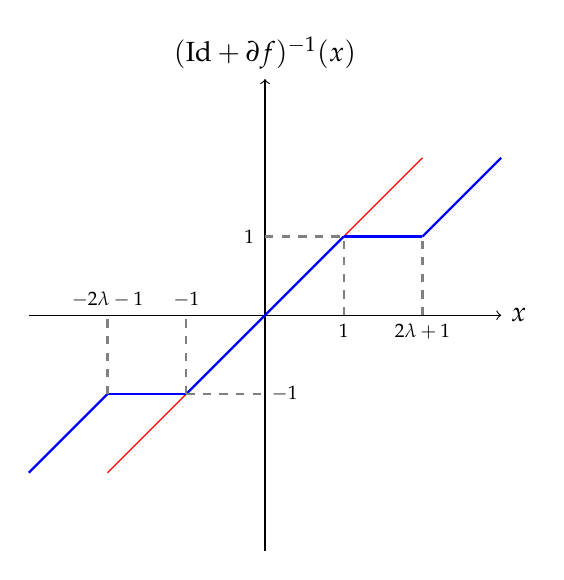
\begin{tikzpicture}
				\draw[->] (-3, 0) -- (3, 0) node[right] {$x$};
				\draw[->] (0, -3) -- (0, 3) node[above] {$(\text{Id} + \partial f)^{-1}(x)$};
				\draw[thin, domain=-2:2, smooth, variable=\x, red] plot ({\x}, {\x});
				\draw[thick, domain=-2:-1, smooth, variable=\x, blue] plot ({\x-1}, {\x});
				\draw[thick, domain=-2:-1, smooth, variable=\y, blue] plot ({\y}, {-1});
				\draw[thick, domain=-1:1, smooth, variable=\x, blue] plot ({\x}, {\x});
				\draw[thick, domain=1:2, smooth, variable=\y, blue] plot ({\y}, {1});
				\draw[thick, domain=1:2, smooth, variable=\x, blue] plot ({\x+1}, {\x});
				
				% Dashed lines
				\path[draw=gray, dashed, thick] (-1,-1) -- (-1,0);
				\path[draw=gray, dashed, thick] (-1,-1) -- (0,-1);
				\path[draw=gray, dashed, thick] (-2,-1) -- (-2,0);
				\path[draw=gray, dashed, thick] (2,0) -- (2,1);
				\path[draw=gray, dashed, thick] (1,0) -- (1,1);
				\path[draw=gray, dashed, thick] (0,1) -- (1,1);
				
				% ticks
				\node[font=\scriptsize,inner sep=1pt,] at (-1, 0.2) {$-1$};
				\node[font=\scriptsize,inner sep=1pt,] at (1, -0.2) {$1$};
				\node[font=\scriptsize,inner sep=1pt,] at (0.25, -1) {$-1$};
				\node[font=\scriptsize,inner sep=1pt,] at (-2, 0.2) {$-2\lambda-1$};
				\node[font=\scriptsize,inner sep=1pt,] at (-0.2, 1) {$1$};
				\node[font=\scriptsize,inner sep=1pt,] at (2, -0.2) {$2\lambda+1$};
			\end{tikzpicture}
	}}
	
	Finally, the fixed points are those that match the identity function (the red line in the previous figure). Those are $[-1,1]$. As we already know, these are the minimums of our original function $f$.
	
\end{document}
